\documentclass[spec, och, labwork]{shiza}
% параметр - тип обучения - одно из значений:
%    spec     - специальность
%    bachelor - бакалавриат (по умолчанию)
%    master   - магистратура
% параметр - форма обучения - одно из значений:
%    och   - очное (по умолчанию)
%    zaoch - заочное
% параметр - тип работы - одно из значений:
%    referat    - реферат
%    coursework - курсовая работа (по умолчанию)
%    diploma    - дипломная работа
%    pract      - отчет по практике
% параметр - включение шрифта
%    times    - включение шрифта Times New Roman (если установлен)
%               по умолчанию выключен
\usepackage{subfigure}
\usepackage{tikz,pgfplots}
\pgfplotsset{compat=1.5}
\usepackage{float}

%\usepackage{titlesec}
\setcounter{secnumdepth}{4}
%\titleformat{\paragraph}
%{\normalfont\normalsize}{\theparagraph}{1em}{}
%\titlespacing*{\paragraph}
%{35.5pt}{3.25ex plus 1ex minus .2ex}{1.5ex plus .2ex}

\titleformat{\paragraph}[block]
{\hspace{1.25cm}\normalfont}
{\theparagraph}{1ex}{}
\titlespacing{\paragraph}
{0cm}{2ex plus 1ex minus .2ex}{.4ex plus.2ex}

% --------------------------------------------------------------------------%


\usepackage[T2A]{fontenc}
\usepackage[utf8]{inputenc}
\usepackage{graphicx}
\graphicspath{ {./images/} }
\usepackage{tempora}

\usepackage[sort,compress]{cite}
\usepackage{amsmath}
\usepackage{amssymb}
\usepackage{amsthm}
\usepackage{fancyvrb}
\usepackage{listings}
\usepackage{listingsutf8}
\usepackage{longtable}
\usepackage{array}
\usepackage[english,russian]{babel}

% \usepackage[colorlinks=true]{hyperref}
\usepackage{url}

\usepackage{underscore}
\usepackage{setspace}
\usepackage{indentfirst} 
\usepackage{mathtools}
\usepackage{amsfonts}
\usepackage{enumitem}
\usepackage{tikz}

\newcommand{\eqdef}{\stackrel {\rm def}{=}}
\newcommand{\specialcell}[2][c]{%
\begin{tabular}[#1]{@{}c@{}}#2\end{tabular}}

\renewcommand\theFancyVerbLine{\small\arabic{FancyVerbLine}}

\newtheorem{lem}{Лемма}

\begin{document}

% Кафедра (в родительном падеже)
\chair{}

% Тема работы
\title{Теория псевдослучайных генераторов}

% Курс
\course{4}

% Группа
\group{431}

% Факультет (в родительном падеже) (по умолчанию "факультета КНиИТ")
\department{факультета КНиИТ}

% Специальность/направление код - наименование
%\napravlenie{09.03.04 "--- Программная инженерия}
%\napravlenie{010500 "--- Математическое обеспечение и администрирование информационных систем}
%\napravlenie{230100 "--- Информатика и вычислительная техника}
%\napravlenie{231000 "--- Программная инженерия}
\napravlenie{100501 "--- Компьютерная безопасность}

% Для студентки. Для работы студента следующая команда не нужна.
% \studenttitle{Студентки}

% Фамилия, имя, отчество в родительном падеже
\author{Окунькова Сергея Викторовича}

% Заведующий кафедрой
% \chtitle{} % степень, звание
% \chname{}

%Научный руководитель (для реферата преподаватель проверяющий работу)
\satitle{доцент} %должность, степень, звание
\saname{И. И. Слеповичев}

% Руководитель практики от организации (только для практики,
% для остальных типов работ не используется)
% \patitle{к.ф.-м.н.}
% \paname{С.~В.~Миронов}

% Семестр (только для практики, для остальных
% типов работ не используется)
%\term{8}

% Наименование практики (только для практики, для остальных
% типов работ не используется)
%\practtype{преддипломная}

% Продолжительность практики (количество недель) (только для практики,
% для остальных типов работ не используется)
%\duration{4}

% Даты начала и окончания практики (только для практики, для остальных
% типов работ не используется)
%\practStart{30.04.2019}
%\practFinish{27.05.2019}

% Год выполнения отчета
\date{2023}

\maketitle

% Включение нумерации рисунков, формул и таблиц по разделам
% (по умолчанию - нумерация сквозная)
% (допускается оба вида нумерации)
% \secNumbering

%-------------------------------------------------------------------------------------------
\tableofcontents

\section{Постановка задачи}

\begin{enumerate}
  \item Сгенерировать псевдослучайную последовательность заданным методом.
  \item Исследовать полученную псевдослучайную последовательность на случайность.
\end{enumerate}

\section{Задачи}

\begin{enumerate}
  \item Сгенерировать последовательность из 10000 случайных чисел из диапазона [0,1]. Исходной программой для генерации ПСЧ может быть программа, созданная в рамках практической работы по данному курсу.
  \item Протестировать статистические свойства последовательности псевдослучайных чисел:
  \begin{center}
    \textbf{Линейный конгруэнтный метод}
  \end{center}
  Матожидание последовательности: 0.50010703125
  
  Среднеквадратичное отклонение последовательности: 0.28852824359442625
  \begin{figure}[H]
    \centering
    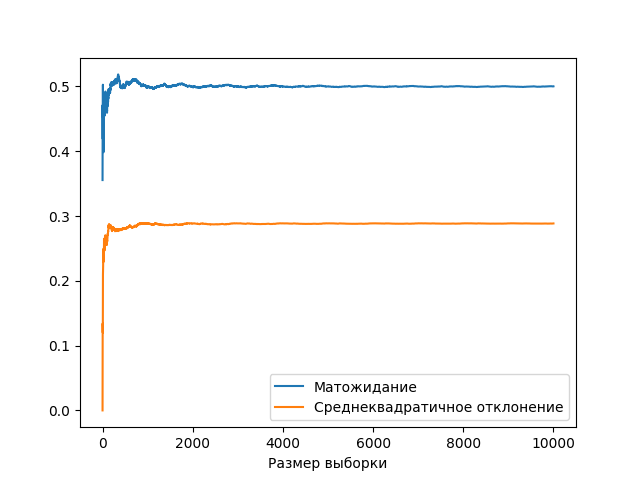
\includegraphics[width=0.6\textwidth]{pic/lc}
    \caption{Зависимость параметров последовательности от ее размеров}
    \label{fig:img1}
  \end{figure}
  \begin{center}
    \textbf{Аддитивный метод}
  \end{center}
  Матожидание последовательности: 0.4959591796875

  Среднеквадратичное отклонение последовательности: 0.2872104606725692
  \begin{figure}[H]
    \centering
    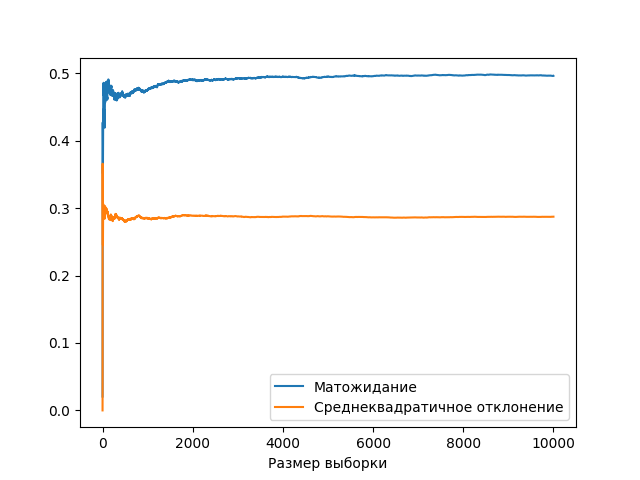
\includegraphics[width=0.6\textwidth]{pic/add}
    \caption{Зависимость параметров последовательности от ее размеров}
    \label{fig:img1}
  \end{figure}
  \begin{center}
    \textbf{Пятипараметрический метод}
  \end{center}
  Матожидание последовательности: 0.50767685546875

  Среднеквадратичное отклонение последовательности: 0.28925578849425804
  \begin{figure}[H]
    \centering
    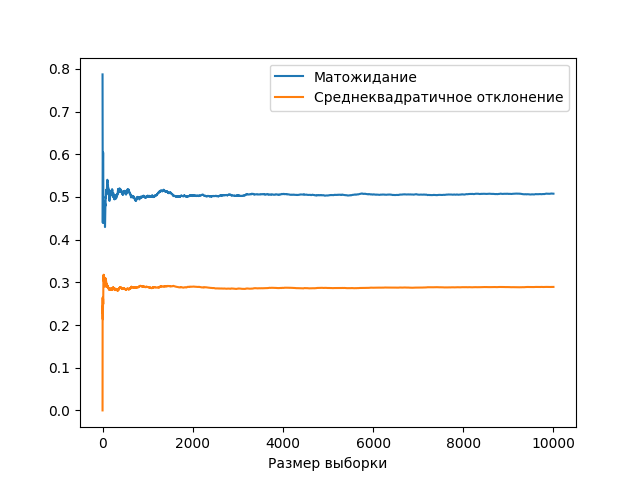
\includegraphics[width=0.6\textwidth]{pic/5p}
    \caption{Зависимость параметров последовательности от ее размеров}
    \label{fig:img1}
  \end{figure}
  \begin{center}
    \textbf{Регистр сдвига с обратной связью (РСЛОС)}
  \end{center}
  Матожидание последовательности: 0.5003677734375

  Среднеквадратичное отклонение последовательности: 0.2893232093627731
  \begin{figure}[H]
    \centering
    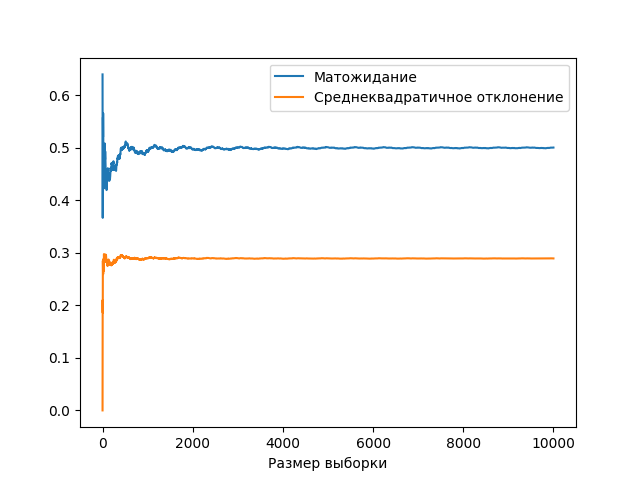
\includegraphics[width=0.6\textwidth]{pic/lfsr}
    \caption{Зависимость параметров последовательности от ее размеров}
    \label{fig:img1}
  \end{figure}
  \begin{center}
    \textbf{Нелинейная комбинация РСЛОС}
  \end{center}
  Матожидание последовательности: 0.49951357421875

  Среднеквадратичное отклонение последовательности: 0.2888325181050929
  \begin{figure}[H]
    \centering
    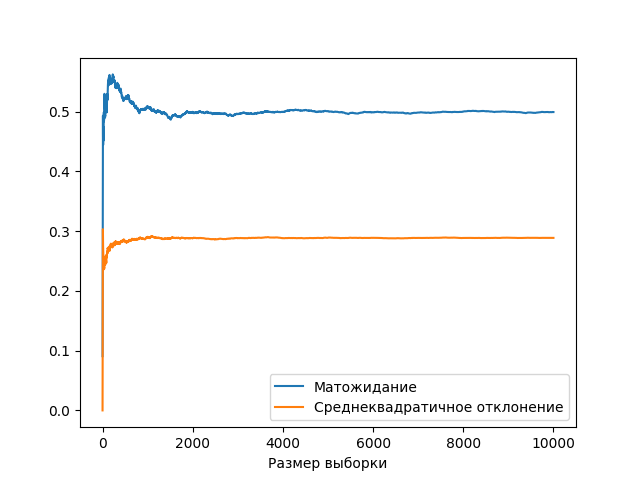
\includegraphics[width=0.6\textwidth]{pic/nfsr}
    \caption{Зависимость параметров последовательности от ее размеров}
    \label{fig:img1}
  \end{figure}
  \begin{center}
    \textbf{Вихрь Мерсенна}
  \end{center}
  Матожидание последовательности: 0.488571875

  Среднеквадратичное отклонение последовательности: 0.28117027311383785
  \begin{figure}[H]
    \centering
    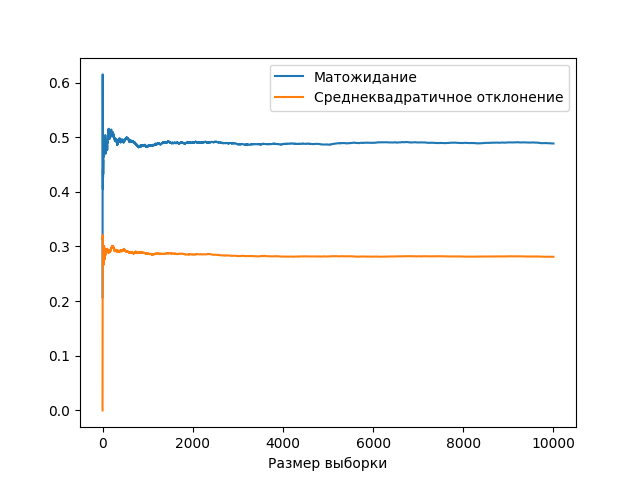
\includegraphics[width=0.6\textwidth]{pic/mt}
    \caption{Зависимость параметров последовательности от ее размеров}
    \label{fig:img1}
  \end{figure}
  \begin{center}
    \textbf{RC4}
  \end{center}
  Матожидание последовательности: 0.4899671875

  Среднеквадратичное отклонение последовательности: 0.28941360272678673
  \begin{figure}[H]
    \centering
    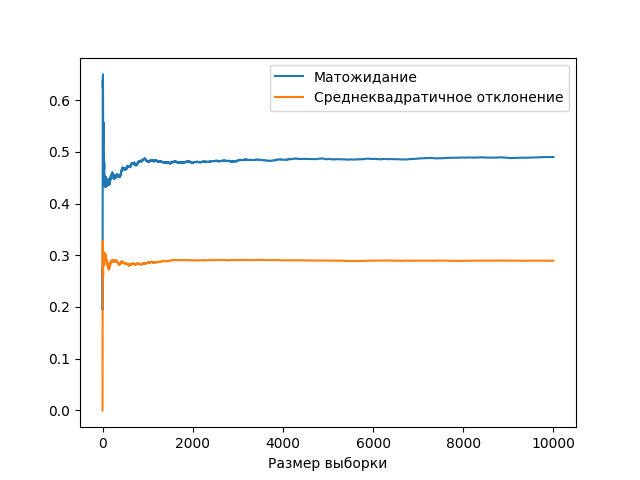
\includegraphics[width=0.6\textwidth]{pic/rc}
    \caption{Зависимость параметров последовательности от ее размеров}
    \label{fig:img1}
  \end{figure}
  \begin{center}
    \textbf{ГПСЧ на основе RSA}
  \end{center}
  Матожидание последовательности: 0.52794599609375

  Среднеквадратичное отклонение последовательности: 0.3225197302247846

  \begin{figure}[H]
    \centering
    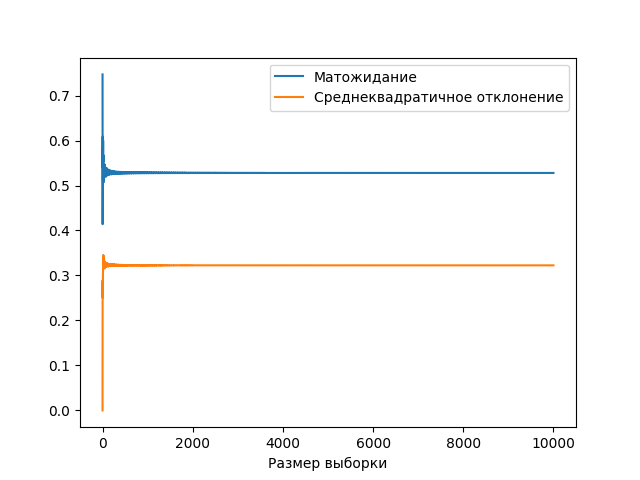
\includegraphics[width=0.6\textwidth]{pic/rsa}
    \caption{Зависимость параметров последовательности от ее размеров}
    \label{fig:img1}
  \end{figure}
  \begin{center}
    \textbf{Алгоритм Блюм-Блюма-Шуба}
  \end{center}
  Матожидание последовательности: 0.38854091796875

  Среднеквадратичное отклонение последовательности: 0.282881865396077
  \begin{figure}[H]
    \centering
    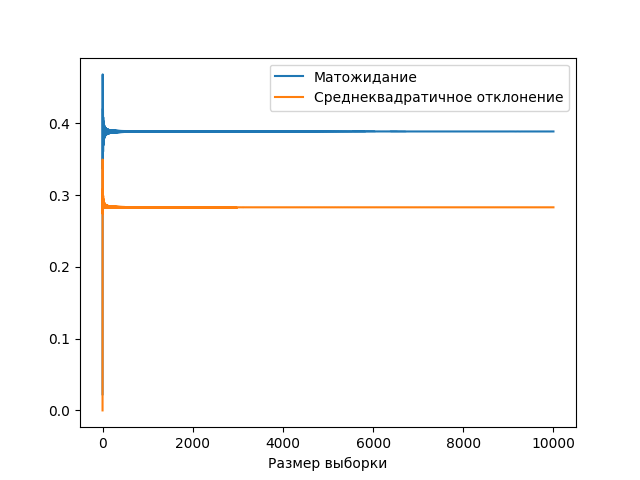
\includegraphics[width=0.6\textwidth]{pic/bbs}
    \caption{Зависимость параметров последовательности от ее размеров}
    \label{fig:img1}
  \end{figure}
\end{enumerate}

\section{Результаты проверки последовательностей на тестах NIST}
\begin{table}[H]
  \resizebox{\textwidth}{!}{%
  \begin{tabular}{|l|l|l|l|l|l|l|l|}
  \hline
   & Хи-квадрат & Серий & Интервалов & Разбиений & Перестановок & Монотонности \\ \hline
  lc   & + & - & + & - & - & - \\ \hline
  add  & + & + & - & + & + & + \\ \hline
  5p   & + & - & + & - & - & -  \\ \hline
  lfsr & + & - & + & - & - & -  \\ \hline
  nfsr & - & - & + & - & - & - \\ \hline
  mt   & - & - & + & - & - & -  \\ \hline
  rc4  & - & - & + & - & - & -  \\ \hline
  rsa  & - & - & + & - & - & -  \\ \hline
  bbs  & - & + & - & - & - & -  \\ \hline
  \end{tabular}%
  }
\end{table}

\end{document}